\documentclass{article} % For LaTeX2e
\usepackage{nips13submit_e,times}
\usepackage{hyperref}
\usepackage{url}
\usepackage{graphicx}

%\documentstyle[nips13submit_09,times,art10]{article} % For LaTeX 2.09


\title{Data Mining for Associations in Biomedical Literature}


\author{
Walton Macey
Department of Computer Science\\
University of Tennessee Knoxville\\
\texttt{wmacey@vols.utk.edu} \\
}


\newcommand{\fix}{\marginpar{FIX}}
\newcommand{\new}{\marginpar{NEW}}

\nipsfinalcopy % Uncomment for camera-ready version

\begin{document}


\maketitle

\begin{abstract}
{\bf Scientific literature relating to the biomedical sciences can typically be reproduced through a comprehensive understanding of a papers four rhetorical elements: Data, Methods, Software and Findings. While a scientific article is not necessarily structured with these 4 subtopics in mind, the DMSF information is essential to properly and efficiently recreate an accurate summarization of a paper’s results. In taking a machine learning approach of extracting these essential aspects from a medical paper, the clear first step involves classifying the body of the article into these 4 categories. With sentences properly classified and grouped according to type, further semantic analysis and data mining can be more easily performed. For example, techniques to summarize these elements would be more effective when aggregating like-minded sentences and providing a summary for each rhetorical category, rather than one summary attempt for entire text body.}
\end{abstract}

\section{Background}
Any scientific paper is formed on fundamental elements of data, methods, software and findings, the connection of these is the basis of a central thesis. To properly verify, analyze or reproduce the results of such a paper requires efficient and accurate extraction of these 4 aspects. Current approaches to identify these elements are often challenging and time consuming. An example of such a project where semantic predications are extracted from text is the Semantic Knowledge Representation project. The base source of the SKR project is a database of 60 million predications extracted from Medline citations, which limits analysis and predications of the project to the data available in Medline citations. There is an apparent need for performing analytics by extracting components from the abstract or body of the paper. In an effort to ease comprehension of complex biomedical literature, I applied machine learning principle to the text comprehension of associations within a subset of medical publications. Focusing on data resulting from a few bimolecular related keywords, the hope is to establish a means of classifying and extracting parts of biomedical article according to its association to Data, Methods, Software or Findings (DMSF).


\section{Approach}
\subsection{Dataset}
The initial goal was to perform contextual analysis on full-text biomedical articles from a topical subset and then develop a model which could accurately predict a sentence or section’s associated element. When difficulties arose in easily acquiring and parsing full text publications relating to our desired subset, the project continued utilizing sentences from a publication’s abstract only, however the approach and techniques were used with plans to later utilize a full-text dataset in the same manner. To start off on the road to build a model which could classify biomedical papers according to DMSF association, we first needed to acquire a large quantity of biomedical articles relating to a few key topics. We used ‘molecular biophysics’, ‘molecular dynamics’, and ‘structural biology’ as keywords for our dataset from the PubMed database. Maintained by the National Center for Biotechnology Information, PubMed comprises more than 27 million citations for biomedical literature. While many articles, journals and publications do have the full text available for free, it is difficult to identify which may have full-texts and to programmatically acquire a large quantity. Because the majority of articles in PubMed Central (PMC) are subject to traditional copyright laws and restrictions, they programmatic means of downloading articles does not allow for downloading in bulk. PMC does have an Open Access subset of over 2 million articles available for text mining purposes, however there was no apparent way to easily search this subset for specific articles after downloading the archive files. After a lengthily download time, the subset was stored in several .tar.gz locations according to alphabetical order and commercial use permission. The developer APIs available are entirely free and include many possible features, however there was a community consensus that the documentation was confusing and lacking in practical application. To prevent abuse and protect the site’s integrity, API calls are limited to 100 every 3 seconds and ask that requests be limited to off-peak hours and weekends. At any sign of abuse, PMC seems to automatically block an IP making too many requests. The apparent challenge was developing a means to download thousands of specific files that have full text available without setting of any flags of abuse. 

\subsection{Acquire Data}
After identifying possible methods and techniques to effectively retrieve the desired dataset we first attempted utilization of a local copy of the Open Access Subset. Downloading the entire OA subset took several hours, and there were many failed efforts to parse each directory for one of our keywords to identify which of the 2 million articles we actually wanted to use. After dismissing this approach, we attempted to create a pull request script using the PubMed documentation as guide. Before moving to far down this complicated path, we stumbled across a third party package called BioPython. 

Utilizing Biopython, all we would need is a list of desired ids and any return type of each article could be acquired. There was still the issue of determining if a paper had the full text available, and how we could acquire only the body of the paper without any other extraneous features to the text (Figures, charts, captions …). We were able to implement a python script using the Entrez module and the esearch function to grab a list of ids according to our keywords. For each pubmed id we could acquire an xml version of each article or a Medline citation, which contains each characteristic of a paper in a structured text format. Manually looking through the first 50 or so xml files, only 2 had full text available and they were structured so differently that there seemed to be no clear way to standardize extracting just the body of the paper. At this point, we decided to shift our analysis and dataset to that of the body of text in each article’s abstract. 

\begin{figure}[h!]
\centering
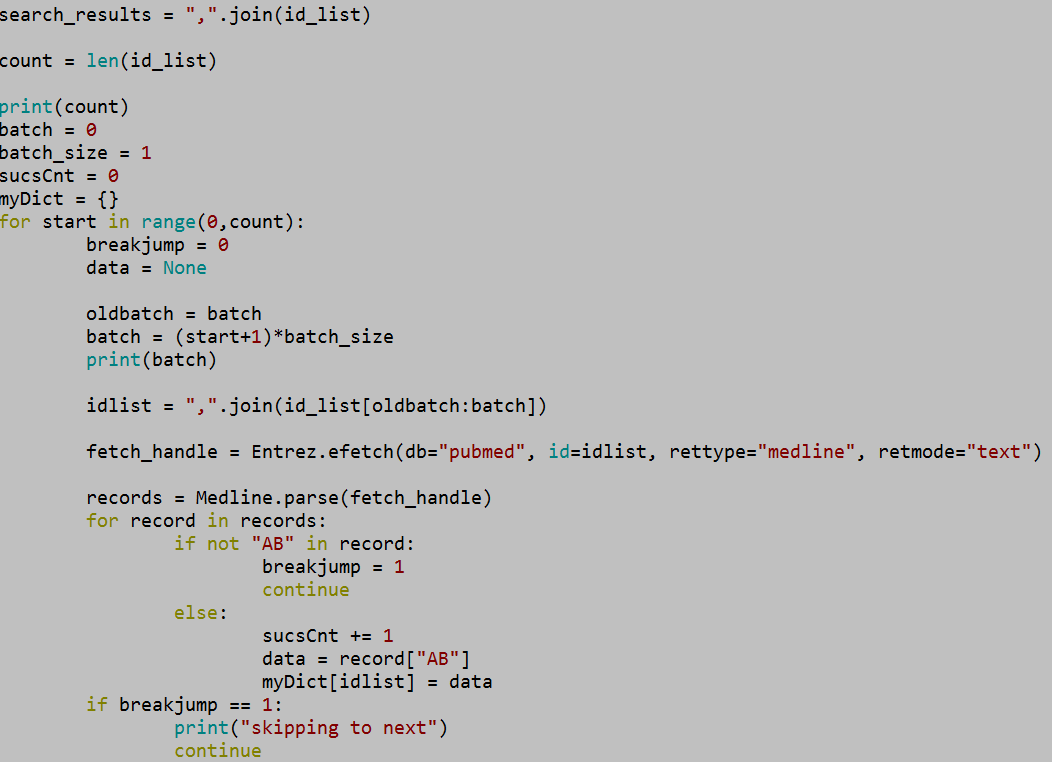
\includegraphics[width=80mm]{Screenshot_107.png}
\caption{Python Script to pull abstract data}
\end{figure}

With this shift in desired outcome, we could develop a python script to fetch PMID’s for specific papers and then fetch only the abstract from the Medline citation. Our script utilized the Entrez and medline module of BioPython and parsed each Medline return for an abstract designation, all while being careful not to exceed the abuse detection limits. The abstracts for all the articles were saved in json format with PMID as the key, for compatibility purposes with Python's Dict class.

\subsection{Classifier}
Now that we had data prepared and ready for input to our model, we began the task of building a supervised learning classifier. Three algorithmic approaches seemed to potentially best suit textual analysis: Naïve Bayes (NB), Support Vector Machines (SVM), and Recurrent Neural Networks (RNN). RNN holds promise as a robust text classifier, but is considered difficult to train and unstable. SVM would be a classifier with higher accuracy, that being said, the classical SVM system is binary, so in order to classify the articles into more than two classes (4) it would require further data manipulation. Naïve Bayes came out as the most obvious first candidate for the model, as it is quickly and efficiently approaches the classification of text from a statistical point of view.

For our model, we harnessed the tools and features of the Natural Language Toolkit (NLTK), a leading platform for language processing within Python Programs. The computational linguistics using Python and this toolkit allow for tokenizing of text, categorizing semantic text and analyzing linguistic structure. Training our model and evaluating our result are done through functions which are part of the Naïve Bayes module of the NLTK package. A classifier based on the Naïve Bayes algorithm, this tool parametrizes the classifier with two probability distributions. The first pdf is the probability of being labeled, or the probability an input (sentence) will receive each label (rhetorical type) without using any information about that particular input’s features (sentence composition). The second pdf is the probability that a feature will receive a given value, based upon the label of the input. In those two definitions, our input would be each sentence, our label would be the rhetorical category type, the value would be the count/frequency and the feature would be the composition of the sentence. 

To overview the python code required to parse the data for training, and then build/evaluate the Naïve Bayes classifier.

1.	Tokenize each abstract into sentences. 
 
\begin{figure}[h!]
\centering
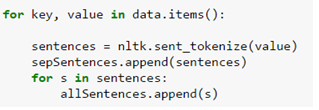
\includegraphics[width=50mm]{Screenshot_127.png}
\caption{Save as sentence array and array of abstracts tokenized into sentences}
\end{figure}

2.	Once training data is prepare, read into feature list
 
\begin{figure}[h!]
\centering
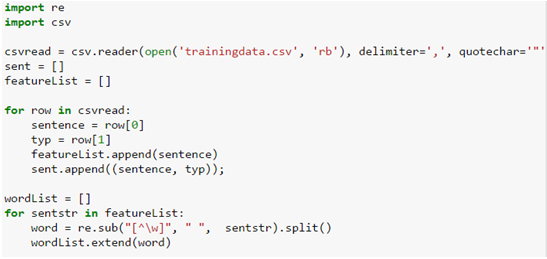
\includegraphics[width=80mm]{Screenshot_126.png}
\caption{Read labeled training data}
\end{figure}

\vspace{20mm}
\vspace{20mm}

3.	Create extract features function to account for word frequency in each class
 
\begin{figure}[h!]
\centering
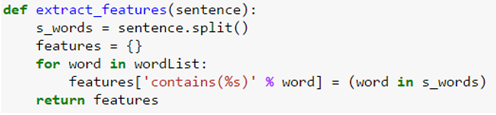
\includegraphics[width=80mm]{Screenshot_125.png}
\caption{Extracts word count according to type in relation to all words}
\end{figure}

4.	Apply features to training set and split test and training data
 
\begin{figure}[h!]
\centering
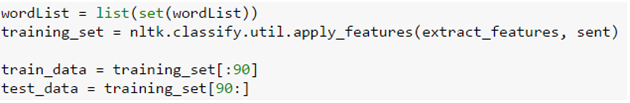
\includegraphics[width=80mm]{Screenshot_124.png}
\caption{Apply features and 90 to 10 training and test split}
\end{figure}

5.	Train model and test predicting power
 
\begin{figure}[h!]
\centering
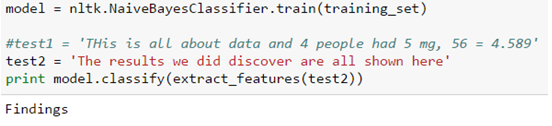
\includegraphics[width=80mm]{Screenshot_123.png}
\caption{Train the NB classifier and spot check with custom sentences}
\end{figure}


\subsection{Training Data}

	To backtrack a little, one of the more time consuming aspects of the classification was building the training data. Through a slow manual classification process and following rules according to observed trends and patterns, we classified approximately 500 sentences as being clearly associated with one type of the DMSF categories. 
    
Here are some keywords and patterns used as a basis for this supervised dataset

\begin{itemize}
\item Findings
\begin{itemize}
\item result, conclusion, find, found, shown, analysis, occurred
\item sentences seen as analysis as a result of some experiment
\item past tense often passive action
\end{itemize}
\item Data
\begin{itemize}
\item data, mg, nm, numbers, concentration, percent, hour, year
\item Numbers with units of measurement
\end{itemize}
\item Methods
\begin{itemize}
\item use, compare, trial, measure, can, evaluate
\item infinitive form of verb
\end{itemize}
\item Software
\begin{itemize}
\item computer, software, program, algorithm, process, model, code
\end{itemize}
\end{itemize}

\vspace{20mm}
\vspace{20mm}

Findings were the most easily identifiable as well as the most frequently found clear classification. Software and to some degree method wore more difficult to identify and less common. These 4 sentences are strong examples for their respective classification. 

\begin{figure}[h!]
\centering
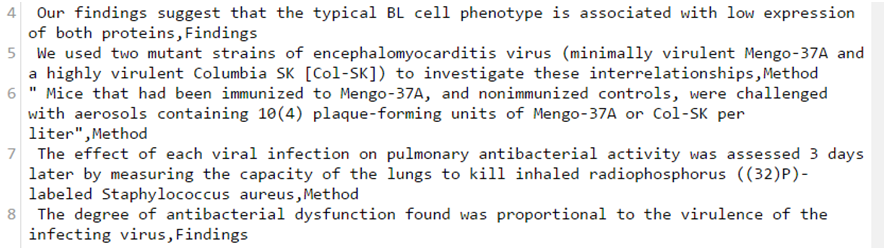
\includegraphics[width=100mm]{Screenshot_122.png}
\caption{Five manually labeled sentences}
\end{figure}
 
Sentence 6 is one which we believed to be a clear example of a Method classification, but it does not appear to follow any keyword indicators or general patterns to indicate so. The sentences classified as ‘Findings’ contain indicators like ‘findings’, ‘found’ and past tense verbs receiving an action (i.e ‘was proportional’).

\begin{figure}[h!]
\centering
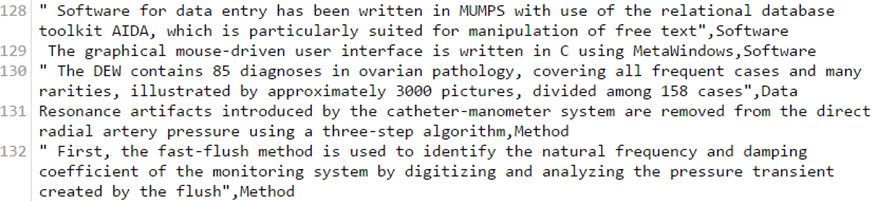
\includegraphics[width=100mm]{Screenshot_121.png}
\caption{Five manually labeled sentences}
\end{figure}

Sometimes, a sentence is obviously of one classification despite containing a keyword common for another. This can be seen in sentence 131, where ‘algorithm’ is present but clearly describes a method or action of the experiment.
 
With 90 percent of the labeled data as training data, the NB classifier can test its classification prowess on the remaining 10 percent of the test data.

\section{Evaluation}


In evaluating the resulting NB classifier, we invoked the ‘nltk.classify.util.accuracy’ function to see how its predictions would fare on the 100 or so remaining sentences. We were impressed to see a resulting accuracy of 92.68 percent. When spot checking the classify function of the model, it seemed to generally correctly classify obvious candidates for each type. However, when given a sentence which could be classified in 1+ ways, the model most often returned a ‘Findings’ designation, even if the sentence most closely associated with two other categories.

\begin{figure}[h!]
\centering
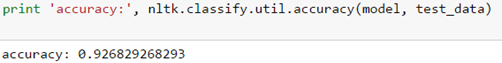
\includegraphics[width=70mm]{Screenshot_120.png}
\caption{Returned value when testing accuracy against test data}
\end{figure}

The NLTK package includes a interesting function which as the name would suggest shows the most informative features to the classifier based on the class with higher and lower probability of that feature.
 
\begin{figure}[h!]
\centering
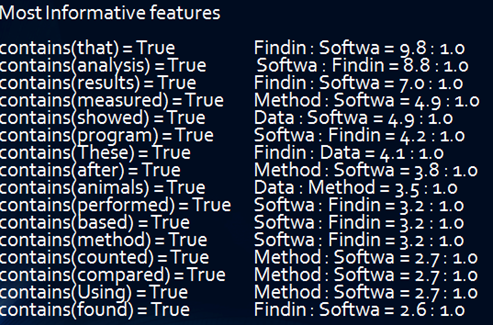
\includegraphics[width=70mm]{Screenshot_119.png}
\caption{Informative features in descending order}
\end{figure}

When ranking these features, some obvious words served as effective predications: {\bf Findings}- results, These, found; {\bf Method}- measured, compared, counted, using; and {\bf Software}- program, perform. Interestingly though, ‘method’ and ‘analysis’ were used as an identifier for ‘Software’ classifications even though for the training data I considered them  ‘Method’ and ‘Finding’ indicators respectively,

\section{Conclusion}

	Moving forward, we do consider this a successful effort and beginning to efficiently identify DMSF associations within a contained subset of medical literature. The entire project feels like a prototyping approach where the next step would be to apply the technique and approach to a full-text data set and to improve the training data and model in the process. At this point, we have successfully identified a way to acquire the entire xml of papers that do contain the full text. We utilized BioPython again and filtering functions native to the Pubmed browser search to identify approximately nine thousand PMIDs of articles relating to our keywords, contained in the Open Access Subset and allowing access to the full-text. With this list of ids, we managed to pull the full xml output for each article, with the remaining task being a comprehensive parse of just the full-text body of the paper. Because the articles do not follow a required formatting or structure, the current bottleneck in the project is finding and effective way to programmatically acquire the clean sentence separated version of the full-text
   
\begin{figure}[h!]
\centering
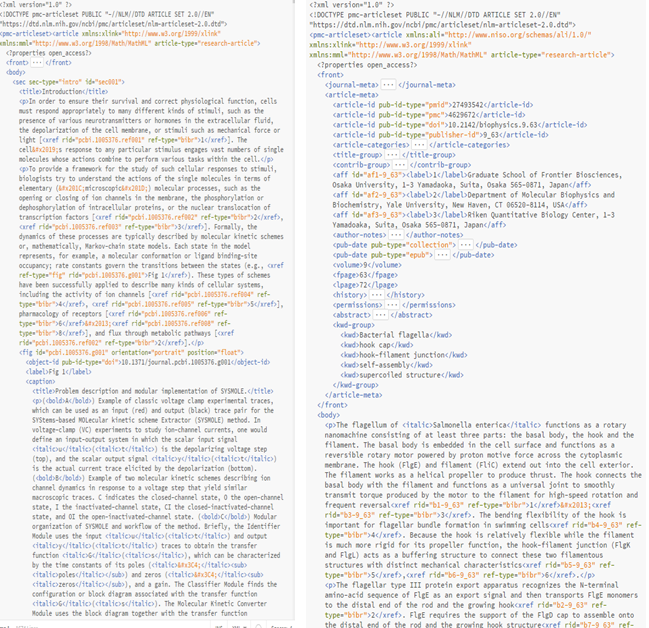
\includegraphics[width=70mm]{Screenshot_118.png}
\caption{Python Script to pull abstract data}
\end{figure}

	With the inclusion of full-text data to our training set, we could increase the size and variety of sentence types for each class. It would also be appropriate to begin to incorporate more features to deciding the classifier’s predictions than just word frequency and sentence composition per type. With the resources made available by having full-text reference, sentence location according to section or the greater context of the whole article can be used as additional indicators. Additionally, due to the nature of a paper being less concise and summary oriented like an abstract, we believe the distribution of the 4 fundamental elements will be more evenly distributed and more clearly aligned with only one category. To further evaluate and improve upon our model, it seems appropriate to try other more difficult algorithmic approaches like Support Vector Machines and Recurrent Neural Network, and find additional means to evaluate the effectiveness of our classifier. Also, because the labeled data for testing and training is created and compiled by 1 person, it would be best to have more individuals create training data to reduce bias in this instance.
Once we have a robust and effective classifier for identifying associations in full-text of biomedical papers we have the foundation for applying further textual analysis to the dataset. With the paper classified accurately into the 4 essentials, we have structured the data in a way such that summarization techniques can be easily utilized and the central thesis of any biomedical paper can be programmatically ascertained in an instant.



\subsubsection*{References}


\small{
[1] Jurafsky, D. (2012) {\it Text Classification and Naive Bayes: The Task of Text Classification}
Stanford University; https://www.stanford.edu/class/cs124/lec/naivebayes.pdf .

[2] Natural Language Toolkit. {\it www.nltk.or}

[3] BioPython. {\it biopython.org }

[4] Agarwal, S. \& Yu, H. (2009) {\it Automatically classifying sentences in full-text biomedical articles}
University of William and Mary.


\end{document}